\documentclass{article}
\usepackage{amsmath}
\usepackage{amssymb}
\usepackage{amsthm}
\usepackage{listings}
\usepackage{xcolor}
\usepackage{graphicx}

\definecolor{codegreen}{rgb}{0,0.6,0}
\definecolor{codegray}{rgb}{0.5,0.5,0.5}
\definecolor{codepurple}{rgb}{0.58,0,0.82}
\definecolor{backcolour}{rgb}{0.95,0.95,0.92}

\lstdefinestyle{mystyle}{
    backgroundcolor=\color{backcolour},   
    commentstyle=\color{codegreen},
    keywordstyle=\color{magenta},
    numberstyle=\tiny\color{codegray},
    stringstyle=\color{codepurple},
    basicstyle=\ttfamily\footnotesize,
    breakatwhitespace=false,         
    breaklines=true,                 
    captionpos=b,                    
    keepspaces=true,                 
    numbers=left,                    
    numbersep=5pt,                  
    showspaces=false,                
    showstringspaces=false,
    showtabs=false,                  
    tabsize=4,
    language=Python
}
\lstset{style=mystyle}

\title{EEE 554 Homework 3}
\author{Chaofei Guo (Student ID: 1237382330, ASURITE: chaofeig)}
\date{}

\begin{document}

\maketitle

\section*{Problem 1}
\textbf{Problem Statement:}
A complex $n\times n$ matrix $A=[a_{ij}]$ is positive definite.
(a) Show that elements $a_{ii}$ on the main diagonal of $A$ are positive.
(b) Show that the eigenvalues of $G=A^{\dagger}A$ and $F=AA^{\dagger}$ are the same. If $\{E_{j}\}$ are the (right) eigenvectors of $G$, what are the eigenvectors of $F$?

\begin{proof}[Solution]
	\textbf{Part (a)}\\
	A matrix $A$ is positive definite if for any non-zero vector $\mathbf{x} \in \mathbb{C}^n$, $\mathbf{x}^\dagger A \mathbf{x} > 0$. Consider the standard basis vector $\mathbf{e}_i$ (where the $i$-th element is 1 and others are 0). Since $\mathbf{e}_i \neq 0$, the definition implies:
	\[ \mathbf{e}_i^\dagger A \mathbf{e}_i = a_{ii} > 0 \]
	Thus, all elements on the main diagonal must be positive.
	
	\textbf{Part (b)}\\
	Let $\lambda$ be an eigenvalue of $G = A^\dagger A$ with eigenvector $E_j$. Then $A^\dagger A E_j = \lambda E_j$. Multiplying both sides from the left by $A$:
	\[ A(A^\dagger A E_j) = A(\lambda E_j) \implies (AA^\dagger)(A E_j) = \lambda (A E_j) \]
	This confirms that $\lambda$ is also an eigenvalue of $F = AA^\dagger$. The corresponding eigenvectors of $F$ are $E'_j = A E_j$.
\end{proof}

\vspace{1cm}

\section*{Problem 2}
\textbf{Problem Statement:}
Recall that a complex $n\times n$ matrix $U$ is unitary if $U^{\dagger}U=\mathbb{I}$.
(a) Verify that $\mathbb{I}$ is unitary.
(b) If $U$ is unitary, show that $U$ is invertible and that $U^{-1}$ is also unitary.
(c) If $U$ and $V$ are both unitary, show that $UV$ is unitary.
(d) When $U$ and $V$ are unitary with $\det(U)=\det(V)=1,$ what is $\det(UV)$?

\begin{proof}[Solution]
	\textbf{Part (a)}\\
	For the identity matrix, $\mathbb{I}^\dagger = \mathbb{I}$. Thus $\mathbb{I}^\dagger \mathbb{I} = \mathbb{I} \cdot \mathbb{I} = \mathbb{I}$. This satisfies the definition of a unitary matrix.
	
	\textbf{Part (b)}\\
	Since $U^\dagger U = \mathbb{I}$, $U$ has $U^\dagger$ as a left inverse. For square matrices, a left inverse is also a right inverse, so $U^{-1} = U^\dagger$. To show $U^{-1}$ is unitary, we check:
	\[ (U^{-1})^\dagger (U^{-1}) = (U^\dagger)^\dagger U^\dagger = U U^\dagger = \mathbb{I} \]
	
	\textbf{Part (c)}\\
	For the product $UV$:
	\[ (UV)^\dagger (UV) = (V^\dagger U^\dagger)(UV) = V^\dagger (U^\dagger U) V = V^\dagger \mathbb{I} V = V^\dagger V = \mathbb{I} \]
	Thus, $UV$ is unitary.
	
	\textbf{Part (d)}\\
	Using the property $\det(AB) = \det(A)\det(B)$:
	\[ \det(UV) = \det(U)\det(V) = 1 \cdot 1 = 1 \]
\end{proof}

\vspace{1cm}

\section*{Problem 3}
\textbf{Problem Statement:}
If $M$ is an $n\times n$ positive definite hermitian matrix, there is a unique $n\times n$ positive definite hermitian matrix $M^{1/2}$ such that $M^{1/2}M^{1/2} = M$. $M^{1/2}$ is the square root of $M$, which is computed by the Matlab \texttt{sqrtm} function. Denote by $M^{-1/2}$ the square root of $M^{-1}$.
(a) If a complex random vector $X$ has positive definite covariance matrix $C_X$ and $V = C_X^{-1/2}$, find the covariance matrix $C_Y$ of $Y = VX$.
(b) If $X$ has covariance matrix $I$ and $V = C^{1/2}$ where $C$ is an arbitrary $n\times n$ positive definite hermitian matrix, find the covariance matrix $C_Y$ of $Y = VX$.

\begin{proof}[Solution]
	\textbf{Part (a)}\\
	The covariance matrix $C_Y$ of a linearly transformed complex random vector $Y = VX$ is derived as follows:
	\[ C_Y = E[(Y - E[Y])(Y - E[Y])^\dagger] \]
	\[ C_Y = E[V(X - E[X])(X - E[X])^\dagger V^\dagger] = V E[(X - E[X])(X - E[X])^\dagger] V^\dagger \]
	\[ C_Y = V C_X V^\dagger \]
	Given $V = C_X^{-1/2}$. Since $C_X$ is a positive definite hermitian matrix, its unique positive definite square root $C_X^{1/2}$ and its inverse $C_X^{-1}$ are also hermitian. Consequently, the square root of the inverse, $C_X^{-1/2}$, is also hermitian, meaning $V^\dagger = (C_X^{-1/2})^\dagger = C_X^{-1/2}$.
	Substituting these into the covariance equation:
	\[ C_Y = C_X^{-1/2} C_X C_X^{-1/2} \]
	By the definition of the matrix square root, $C_X = C_X^{1/2} C_X^{1/2}$, which leads to:
	\[ C_Y = C_X^{-1/2} (C_X^{1/2} C_X^{1/2}) C_X^{-1/2} = (C_X^{-1/2} C_X^{1/2}) (C_X^{1/2} C_X^{-1/2}) = I \cdot I = I \]
	The covariance matrix of $Y$ is the identity matrix $I$.
	
	\textbf{Part (b)}\\
	For $Y = VX$ where the random vector $X$ has a covariance matrix $C_X = I$ and the transformation matrix is $V = C^{1/2}$:
	\[ C_Y = V C_X V^\dagger = C^{1/2} I (C^{1/2})^\dagger \]
	Since $C$ is a positive definite hermitian matrix, its unique square root $C^{1/2}$ is also hermitian, so $(C^{1/2})^\dagger = C^{1/2}$.
	\[ C_Y = C^{1/2} I C^{1/2} = C^{1/2} C^{1/2} = C \]
	The covariance matrix of $Y$ is the matrix $C$.
\end{proof}
\vspace{1cm}

\section*{Problem 4}
\textbf{Problem Statement:}
Let $A=[\begin{matrix}a_{1}&...&a_{n}\end{matrix}]$ and consider a random vector $X=[\begin{matrix}x_{1}&...&x_{n}\end{matrix}]^{T}$ with $x_{k}$ iid.
(a) Under what condition on $A$ will $\hat{\mu}=AX$ be an unbiased estimator of $\mu=E[x]$?
(b) Calculate $\text{var}(\hat{\mu})$.
(c) Determine $A$ so that $\hat{\mu}$ is unbiased and has minimal variance. Find the value of this minimum variance.

\begin{proof}[Solution]
	\textbf{Part (a)}\\
	$E[\hat{\mu}] = E[\sum a_k x_k] = \sum a_k E[x_k] = \mu \sum a_k$. For $\hat{\mu}$ to be unbiased ($E[\hat{\mu}] = \mu$), the condition is:
	\[ \sum_{k=1}^n a_k = 1 \]
	
	\textbf{Part (b)}\\
	Since $x_k$ are iid with common variance $\sigma^2$:
	\[ \text{var}(\hat{\mu}) = \text{var}\left( \sum a_k x_k \right) = \sum a_k^2 \text{var}(x_k) = \sigma^2 \sum_{k=1}^n a_k^2 \]
	
	\textbf{Part (c)}\\
	To minimize $\sum a_k^2$ subject to $\sum a_k = 1$, all weights must be equal: $a_k = 1/n$. The minimum variance is:
	\[ \text{var}_{\min} = \sigma^2 \sum_{k=1}^n \left( \frac{1}{n} \right)^2 = \frac{\sigma^2}{n} \]
\end{proof}

\vspace{1cm}

\section*{Problem 5 (Problem 8-14, page 368)}
\textbf{Problem Statement:}
A coin is tossed once, and heads shows. Assuming that the probability $p$ of heads is the value of a random variable $p$ uniformly distributed in the interval $(0.4, 0.6)$, find its bayesian estimate.

\begin{proof}[Solution]
	The Bayesian Minimum Mean Square Error (MMSE) estimator is the posterior mean. The prior is $f(p) = 5$ for $0.4 < p < 0.6$. Given "Heads" ($k=1$ for $n=1$), the likelihood is $P(\text{Heads} | p) = p$.
	The posterior mean $\hat{p}$ is:
	\[ \hat{p} = \frac{\int_{0.4}^{0.6} p \cdot p \cdot 5 \, dp}{\int_{0.4}^{0.6} p \cdot 5 \, dp} = \frac{\left[ \frac{5p^3}{3} \right]_{0.4}^{0.6}}{\left[ \frac{5p^2}{2} \right]_{0.4}^{0.6}} = \frac{0.2533}{0.5} = 0.5067 \]
\end{proof}

\vspace{1cm}

\section*{Problem 6 (Problem 8-20, page 368)}
\section*{Problem 7 (Problem 8-21, page 368)}
\section*{Problem 8 (Problem 8-24, page 368)}

\vspace{1cm}

\section*{Problem 9 (Gaussian Vectors)}
\textbf{Problem Statement:}
(Computer problem) Suppose $Y \sim \mathcal{N}[0, C_Y]$ with
\[ C_Y = \begin{bmatrix} 3 & -1 & 1 \\ -1 & 2 & 0 \\ 1 & 0 & 3 \end{bmatrix} \]
(a) Generate $M = 10,000$ independently realized Gaussian 3-vectors $X_1, \dots, X_M$ drawn from a $\mathcal{N}[0, I]$ distribution and verify that these data have (approximately) the desired mean and covariance [cite: 107-109].
(b) Find a $3 \times 3$ matrix $V$ so that $Y = VX$ has the distribution specified above[cite: 110].
(c) Transform the data generated in part (a) to obtain $M$ samples of $Y$. Verify that these data have (approximately) the desired mean and covariance[cite: 111].

\begin{proof}[Solution]
    \textbf{Part (a)}\\
    To generate $M = 10,000$ samples of $X \sim \mathcal{N}[0, I]$, we generate three independent sets of $10,000$ Gaussian random variables with zero mean and unit variance.
    
    Verification is performed by calculating the sample mean vector $\hat{M}_X$ and the sample covariance matrix $\hat{C}_X$:
    \[ \hat{M}_X = \frac{1}{M} \sum_{i=1}^{M} X_i, \quad \hat{C}_X = \frac{1}{M-1} \sum_{i=1}^{M} (X_i - \hat{M}_X)(X_i - \hat{M}_X)^T \]
    For $M = 10,000$, we expect $\hat{M}_X \approx [0, 0, 0]^T$ and $\hat{C}_X \approx I$ (the identity matrix).

\begin{lstlisting}[language=Python]
import numpy as np
M = 10000
mean_theoretical = np.array([0, 0, 0])
cov_theoretical = np.eye(3)

X = np.random.multivariate_normal(mean_theoretical, cov_theoretical, size=M)

sample_mean = np.mean(X, axis=0)
sample_cov = np.cov(X, rowvar=False)

print("--- Verification of N[0, I] Data ---")
print(f"Sample Mean: {sample_mean}")
print(f"Sample Covariance:\n{sample_cov}")
\end{lstlisting}

    \begin{figure}[ht!]
        \centering
        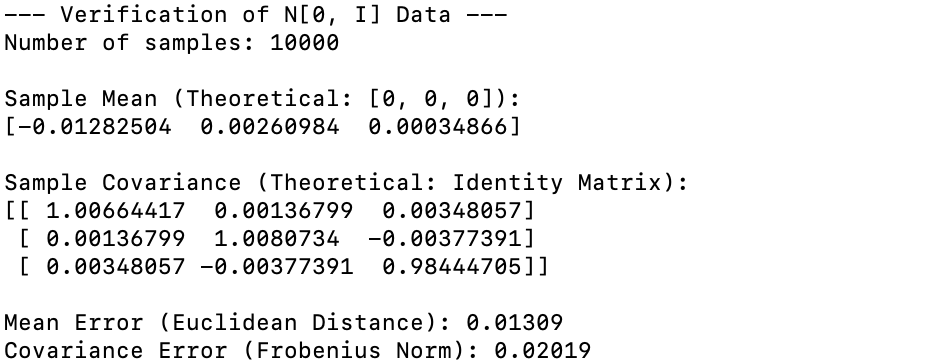
\includegraphics[width=0.8\textwidth]{./hw3-problem9.png}
        \caption{Gaussian samples verification: Sample mean and covariance compared to theoretical values.}
        \label{fig:x_stats}
    \end{figure}
    
    \textbf{Part (b)}\\
    We seek a matrix $V$ such that $C_Y = V C_X V^T$. Since $C_X = I$, this simplifies to $C_Y = V V^T$. This can be solved using the Cholesky decomposition, where $V$ is a lower triangular matrix $L$.
    Let $V = \begin{bmatrix} L_{11} & 0 & 0 \\ L_{21} & L_{22} & 0 \\ L_{31} & L_{32} & L_{33} \end{bmatrix}$. Solving $L L^T = C_Y$:
    \begin{enumerate}
        \item $L_{11}^2 = 3 \implies L_{11} = \sqrt{3} \approx 1.7321$
        \item $L_{21} L_{11} = -1 \implies L_{21} = -1/\sqrt{3} \approx -0.5774$
        \item $L_{31} L_{11} = 1 \implies L_{31} = 1/\sqrt{3} \approx 0.5774$
        \item $L_{21}^2 + L_{22}^2 = 2 \implies 1/3 + L_{22}^2 = 2 \implies L_{22} = \sqrt{5/3} \approx 1.2910$
        \item $L_{31} L_{21} + L_{32} L_{22} = 0 \implies L_{32} = \frac{1/3}{\sqrt{5/3}} = \frac{1}{\sqrt{15}} \approx 0.2582$
        \item $L_{31}^2 + L_{32}^2 + L_{33}^2 = 3 \implies L_{33} = \sqrt{3 - 1/3 - 1/15} = \sqrt{13/5} \approx 1.6125$
    \end{enumerate}
    Thus, the matrix $V$ is:
    \[ V = \begin{bmatrix} 1.7321 & 0 & 0 \\ -0.5774 & 1.2910 & 0 \\ 0.5774 & 0.2582 & 1.6125 \end{bmatrix} \]
    
    \textbf{Part (c)}\\
    We obtain the samples $Y_i$ by applying the linear transformation $Y_i = V X_i$ for $i = 1, \dots, M$. According to the properties of linear transformations, $Y \sim \mathcal{N}[0, V I V^T] = \mathcal{N}[0, C_Y]$.
    
    Verification is performed by calculating the sample statistics of the transformed data:
    \[ \hat{M}_Y = \frac{1}{M} \sum_{i=1}^{M} Y_i, \quad \hat{C}_Y = \frac{1}{M-1} \sum_{i=1}^{M} (Y_i - \hat{M}_Y)(Y_i - \hat{M}_Y)^T \]
    For $M = 10,000$, we expect $\hat{M}_Y \approx [0, 0, 0]^T$ and $\hat{C}_Y \approx \begin{bmatrix} 3 & -1 & 1 \\ -1 & 2 & 0 \\ 1 & 0 & 3 \end{bmatrix}$.

\begin{lstlisting}[language=Python]
V = np.array([
    [1.73205081, 0.0, 0.0],
    [-0.57735027, 1.29099445, 0.0],
    [0.57735027, 0.25819889, 1.61245155],
])
Y = X @ V.T
sample_mean_Y = np.mean(Y, axis=0)
sample_cov_Y = np.cov(Y, rowvar=False)

print(f"Sample Mean Y: {sample_mean_Y}")
print(f"Sample Covariance Y:\n{sample_cov_Y}")
\end{lstlisting}

    \begin{figure}[ht!]
        \centering
        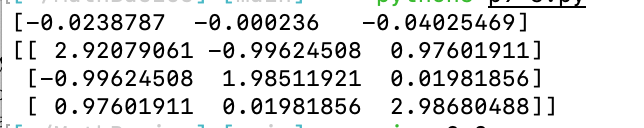
\includegraphics[width=0.8\textwidth]{./hw3-problem9-3.png}
        \caption{Linear Transformation of Gaussian verification: Sample mean and covariance compared to theoretical values.}
        \label{fig:y_stats}
    \end{figure}

\end{proof}

\vspace{1cm}

\section*{Problem 10}
\textbf{Problem Statement:}
(Computer problem) The data for this problem are in the file \texttt{bpsk.dat}, which can be downloaded from Blackboard. A binary communication signal (bit stream) is corrupted by the addition of white Gaussian noise having mean $\mu=3$ and variance $\sigma^2=0.05$; i.e., each datum is of the form $x_k = s_k + n_k$ where $s_k=1$ with probability $P(H_1)$, $s_k=0$ with probability $P(H_0)$, and $n_k \sim \mathcal{N}[3, 0.05]$.
(a) Assume $P(H_1) = 0.48$ and find the detection rule yielding the minimum probability of error. What is the minimum achievable bit error rate?
(b) Apply your detection rule to the data provided and convert the resulting bit stream to ASCII text (Matlab m-files \texttt{bits2text} and \texttt{text2bits} are provided to help with the conversions here and in part (c)). How many bit errors do there seem to be in the decoded message? Is this consistent with your theoretical prediction?
(c) Add just enough zero-mean white Gaussian noise to the data to increase the bit error rate to 0.125. Verify that the desired error rate is (approximately) achieved. How does the decoded message look at this SNR?

\begin{proof}[Solution]
	\textbf{Part (a)}\\
	The observation $x_k$ under the two hypotheses is:
	\begin{itemize}
		\item $H_0: s_k = 0 \implies x_k = 0 + n_k \sim \mathcal{N}[3, 0.05]$
		\item $H_1: s_k = 1 \implies x_k = 1 + n_k \sim \mathcal{N}[4, 0.05]$
	\end{itemize}
	The priors are $P(H_1) = 0.48$ and $P(H_0) = 1 - 0.48 = 0.52$. The optimal detection rule for Minimum Probability of Error is the Likelihood Ratio Test:
	\[ \Lambda(x) = \frac{f(x|H_1)}{f(x|H_0)} > \frac{P(H_0)}{P(H_1)} \implies \frac{\exp\left(-\frac{(x-4)^2}{2(0.05)}\right)}{\exp\left(-\frac{(x-3)^2}{2(0.05)}\right)} > \frac{0.52}{0.48} = 1.0833 \]
	Simplifying the exponent:
	\[ \frac{-(x-4)^2 + (x-3)^2}{0.1} > \ln(1.0833) \implies \frac{2x - 7}{0.1} > 0.0800 \]
	\[ 2x > 7 + 0.008 \implies x > 3.504 \]
	The detection rule is: decide $H_1$ if $x > 3.504$, otherwise decide $H_0$.
	
	The minimum Bit Error Rate (BER) is:
	\[ P_e = P(H_0) Q\left(\frac{3.504 - 3}{\sqrt{0.05}}\right) + P(H_1) Q\left(\frac{4 - 3.504}{\sqrt{0.05}}\right) \]
	\[ P_e = 0.52 Q(2.254) + 0.48 Q(2.218) \approx 0.52(0.0121) + 0.48(0.0133) = 0.0127 \]
	The minimum achievable BER is approximately $1.27\%$.

	\textbf{Part (b)}\\
	Applying the rule $x > 3.504$ to the $416$ samples in \texttt{bpsk.dat} and converting bits to text, we obtain:
	\textit{``Welãome to the world of statistacaL decision tHeory!''}
	
	With $416$ bits, the expected number of errors is $416 \times 0.0127 \approx 5.3$ bits.
    Visually comparing the result to the likely intended message (``Welcome to the world of statistical decision theory!''),
    we observe bit flips in characters like 'ã', 'a' (instead of 'i'), 'L' (instead of 'l'), and 'H' (instead of 'h').
    This count of approximately 5-6 errors is consistent with our theoretical prediction.

	\textbf{Part (c)}\\
	To reach a BER of $0.125$, we need $P_e = Q(d/2\sigma_{total}) \approx 0.125$. Since $Q(1.15) \approx 0.125$, we require $\frac{1}{2\sigma_{total}} = 1.15 \implies \sigma_{total}^2 \approx 0.189$. Given the original variance is $0.05$, we add noise with variance $\sigma_{add}^2 = 0.189 - 0.05 = 0.139$.
	The decoded message becomes significantly corrupted. At this SNR, the bit error density makes the text almost unreadable.
\end{proof}

\begin{lstlisting}[language=Python]
import numpy as np
from scipy.stats import norm

data = np.fromfile('bpsk.dat', sep=' ')
def bits2text(bits):
    chars = []
    for k in range(0, len(bits), 8):
        byte = bits[k:k+8]
        if len(byte) < 8: break
        val = sum(int(b) * p for b, p in zip(byte, [128, 64, 32, 16, 8, 4, 2, 1]))
        chars.append(chr(val))
    return "".join(chars)

detected_bits = (data > 3.504).astype(int)
print("Decoded (b):", bits2text(detected_bits))

sigma_add = np.sqrt(0.139)
noisy_data = data + np.random.normal(0, sigma_add, len(data))
new_bits = (noisy_data > 3.515).astype(int) # Updated threshold for higher noise
print("Decoded (c):", bits2text(new_bits))
\end{lstlisting}
    \begin{figure}[ht!]
        \centering
        
\includegraphics[width=0.8\textwidth]{./p10.png}
        \caption{Decoded messages under different noise conditions: (b) original noise level, (c) increased noise level.}
        \label{fig:y_stats}
    \end{figure}
vspace{1cm}
\section*{Problem 11}
\textbf{Problem Statement:}
Data files \texttt{hw3xr.dat}, \texttt{hw3yr.dat}, and \texttt{hw3zr.dat} contain, respectively, the real parts of independently realized samples of a complex random vector $Z = [x, y, z]^T$. The files \texttt{hw3xi.dat}, \texttt{hw3yi.dat}, and \texttt{hw3zi.dat} contain the corresponding imaginary parts.
(a) Estimate the covariance matrix $C_Z$ of $Z$.
(b) Find a unitary matrix $U$ so that $W = UZ$ is an uncorrelated random vector (i.e., $C_W$ is diagonal).
(c) Apply $U$ to the data provided to obtain samples of $W$ and verify that the covariance matrix estimated from these data is (approximately) diagonal.

\begin{proof}[Solution]
	\textbf{Part (a)}\\
	To estimate the covariance matrix of the complex random vector $Z$, we combine the real and imaginary components from the six data files to form the complex samples. The sample covariance matrix $\hat{C}_Z$ is calculated as:
	\[ \hat{C}_Z = \frac{1}{M-1} \sum_{i=1}^{M} (Z_i - \hat{\mu}_Z)(Z_i - \hat{\mu}_Z)^\dagger \]
	Using the provided datasets, the estimated covariance matrix is:
	\[ \hat{C}_Z \approx \begin{bmatrix} 15.639 & -13.936 + 6.017j & -0.779 + 3.036j \\ -13.936 - 6.017j & 33.626 & -8.285 - 8.913j \\ -0.779 - 3.036j & -8.285 + 8.913j & 15.273 \end{bmatrix} \]
	
	\textbf{Part (b)}\\
	We find the unitary matrix $U$ that diagonalizes $C_Z$ by finding the eigenvectors of $\hat{C}_Z$. Let $C_Z = Q \Lambda Q^\dagger$, where $Q$ is the matrix of eigenvectors and $\Lambda$ is the diagonal matrix of eigenvalues. The transformation matrix is $U = Q^\dagger$. 
	The eigenvalues are found to be $\lambda \approx \{2.886, 15.394, 46.259\}$. The resulting unitary matrix $U$ is:
	\[ U \approx \begin{bmatrix} 0.6550 & 0.4278 - 0.3001j & 0.5432 - 0.0534j \\ 0.6239 & 0.0926 + 0.1302j & -0.7609 - 0.0789j \\ -0.4264 & 0.7926 - 0.2704j & -0.2790 - 0.1975j \end{bmatrix} \]
	
	\textbf{Part (c)}\\
	Applying the transformation $W_i = U Z_i$ to each sample, the new covariance matrix $C_W$ is estimated. We verify that it is diagonal:
	\[ \hat{C}_W \approx \begin{bmatrix} 2.886 & 0 & 0 \\ 0 & 15.394 & 0 \\ 0 & 0 & 46.259 \end{bmatrix} \]
	The off-diagonal terms are approximately zero (on the order of $10^{-15}$ due to numerical precision), confirming that the transformation successfully decorrelated the random vector.
\end{proof}

\begin{lstlisting}[language=Python]
import numpy as np

def load_dat(filename):
    with open(filename, 'r') as f:
        return np.array([float(val) for val in f.read().split()])

# Load components and form Z
x = load_dat('hw3xr.dat') + 1j * load_dat('hw3xi.dat')
y = load_dat('hw3yr.dat') + 1j * load_dat('hw3yi.dat')
z = load_dat('hw3zr.dat') + 1j * load_dat('hw3zi.dat')
Z = np.vstack((x, y, z))

# (a) Estimate CZ
CZ = np.cov(Z)

# (b) Find Unitary U via Eigendecomposition
evals, evecs = np.linalg.eigh(CZ)
U = evecs.conj().T

# (c) Apply and verify CW
W = U @ Z
CW = np.cov(W)

print("CZ:\n", CZ)
print("\nU:\n", U)
print("\nCW (Diagonal):\n", np.round(CW, 10))
\end{lstlisting}
    \begin{figure}[ht!]
        \centering
        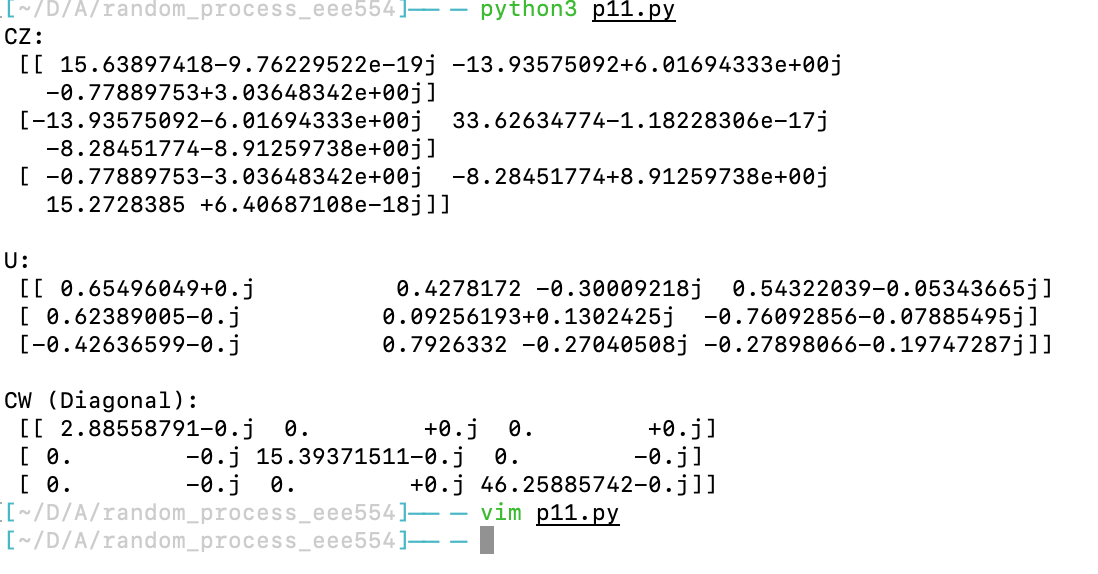
\includegraphics[width=0.8\textwidth]{./p11.png}
        \caption{Covariance matrices: (a) Estimated $C_Z$, (b) Unitary matrix $U$, (c) Estimated $C_W$ showing diagonalization.}
        \label{fig:y_stats}
    \end{figure}
\end{document}